\documentclass[11pt]{article}

\usepackage[letterpaper,margin=0.75in]{geometry}
\usepackage{booktabs}
\usepackage{graphicx}
\usepackage{listings}
\usepackage{fixltx2e}
\usepackage{verbatim}
\usepackage{color}

\definecolor{dkgreen}{rgb}{0,0.6,0}
\definecolor{gray}{rgb}{0.5,0.5,0.5}
\definecolor{mauve}{rgb}{0.58,0,0.82}
\definecolor{orange}{RGB}{255,119,0}
\definecolor{purple2}{RGB}{153,0,153}

\setlength{\parindent}{1.4em}

\begin{document}

\lstset{
  language=Python,
  basicstyle=\small\ttfamily, % print whole listing small
  keywordstyle=\color{orange},
  keywordstyle={[2]\color{purple2}},
  identifierstyle=,           % nothing happens
  commentstyle=\color{dkgreen},% green comments
  stringstyle=\ttfamily\color{mauve},      % typewriter type for strings
  showstringspaces=false,     % no special string spaces
  numbers=left,
  numberstyle=\tiny\color{gray},
  numbersep=5pt,
  frame=tb,
}

\title{CS460 Lab 3 Report: Congestion Control}

\author{Michael K. Eagar}

\date{March 24rd, 2014}

\maketitle

\section{Congestion Control Implementation - TCP Tahoe}

I used my Reliable Transport Protocol implementation as the basis for implementing Congestion Control using the TCP Tahoe model. My implementation is saved in the file \textit{my\_RTP.py}. I needed to change my \textit{transfer.py} file as well, in order to use the Simulator scheduler to schedule different events to start at different times. I modified the \textit{transfer.py} file to add the window initialization method as a scheduled event. I also implemented new versions of \textit{transfer.py} to handle more than one file transfer (two and five flows each) at a time. These are saved as \textit{transfer2.py} and \textit{transfer5.py}. To begin, I implemented \textit{Slow Start}, the \textit{Slow Start Threshold}, \textit{Additive Increase}, and loss event handling:\\

\indent \textbf{Slow Start} - At the start of the connection, or after any kind of loss event, set \textit{cwnd} (congestion window) to 1 MSS. Every time the sender receives an ACK for new data, increment \textit{cwnd} by the number of new bytes of data acknowledged.\\
\indent \textbf{Threshold} - Stop \textit{Slow Start} when \textit{cwnd} exceeds or equals the threshold. Start with a threshold of 100,000 bytes (100 packets).\\
\indent \textbf{Additive Increase} - Once \textit{cwnd} is larger than the threshold, use \textit{additive increase}. Every time the sender receives an ACK for new data, increment \textit{cwnd} by MSS * b / \textit{cwnd}, where MSS is the maximum segment size (1000 bytes) and b is the number of new bytes acknowledged.\\
\indent \textbf{Loss Event Handling} - When a loss event is detected (a timeout), set the threshold to the maximum of \textit{cwnd} divided by 2, and MSS, and set cwnd to 1 MSS.\\\\

My implementation of these features mainly involved adding a few lines of code to my \textit{slide\_window()} and \textit{retransmit} methods. My \textit{slide\_window()} method now reads as follows:

\lstinputlisting[breaklines = true, firstline = 86, lastline = 116, caption = slide\_window()]{./my_rtp.py}
\vspace{0.25cm}
The \textit{retransmit()} method is now:
\lstinputlisting[breaklines = true, firstline = 174, lastline = 189, caption = retransmit()]{./my_rtp.py}
\vspace{0.25cm}

After making these changes to my code and implementing the features for TCP Tahoe Congestion Control, I needed to add the ability to collect the data necessary to verify that my implementation of the new features was working correctly. In order to do this, I modified Dr. Zappala's \textit{tcppacket.py} to allow the TCP packet to keep track of which flow it was a part of, implemented some new methods in \textit{sim.py} to allow for exporting transfer rate and packet loss data, and additional functionality in \textit{link.py} and \textit{my\_rtp.py} to export queue data and congestion window data.\\
\\
The TCP packets now keep track of a new variable called \textit{flow\_id} that can be referenced to determine which flow they were part of. The rate, packet loss, queue, and congestion window data are all exported to individual files to make it easier to parse the data and plot the various graphs that are shown below. It was somewhat challenging for me to put the method calls in the correct places in order to get the proper data I needed to be able to show that my implmentation was working correctly, but I was able to get it to work after quite a bit of trial and error.
\vspace{0.25cm}

\section{Experiments}

To run the experiments that were required in the lab specification I used the \textit{transfer1.py}, \textit{transfer2.py}, and \textit{transfer5.py} scripts that I had set up earlier. Each is set up to transfer the same number of files as is specified in the file names. I had to change them to allow the multiple file transfers and for them to have each transferred file saved with a different name in order to verify that they all transferred correctly. The network is set up with bandwidth of 10 Mbps and a propagation delay of 10 ms. For the two and five flow networks, the queue size was set to 100 packets, because there would be loss when transferring two or five 1 MB files. For the one flow network, however, I needed to set the queue as 80 in order to see any loss.  I also ran the one flow experiment with a queue size of 100, for comparison.
\\
\textbf{Experiment 1} required the transferring of a 1 MB file over the link. The exported data for Experiement 1 is saved in the \textit{lab3/1\_data} directory, in the text files that begin with \textbf{1\-}. Figures 1 through 8 show the plots constructed from the data received from this experiment.
\vspace{0.25cm}
\textit{Figure 1 - Queue Size vs Time with Max Queue Size of 80}
\\
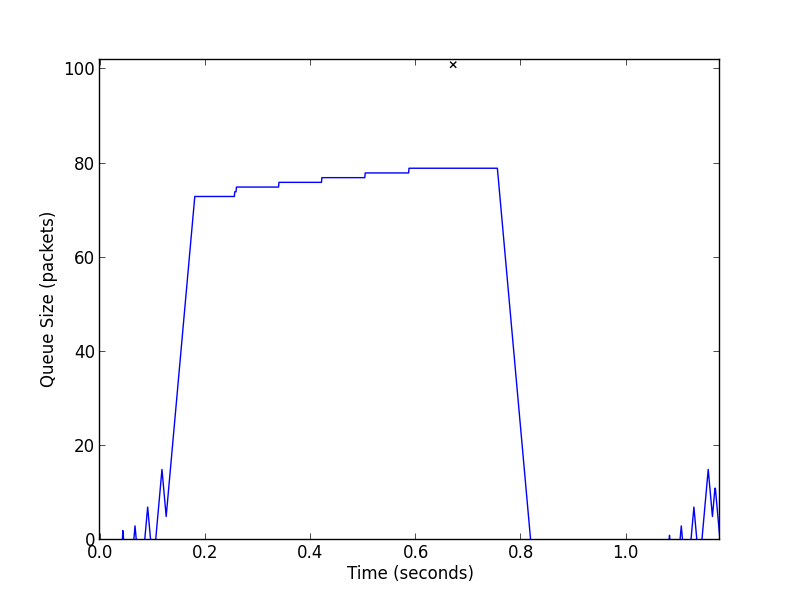
\includegraphics[width=13cm]{1_data/1-queue_q80}
\vspace{0.25cm}

\textit{Figure 2 - Queue Size vs Time with Max Queue Size of 100}
\\
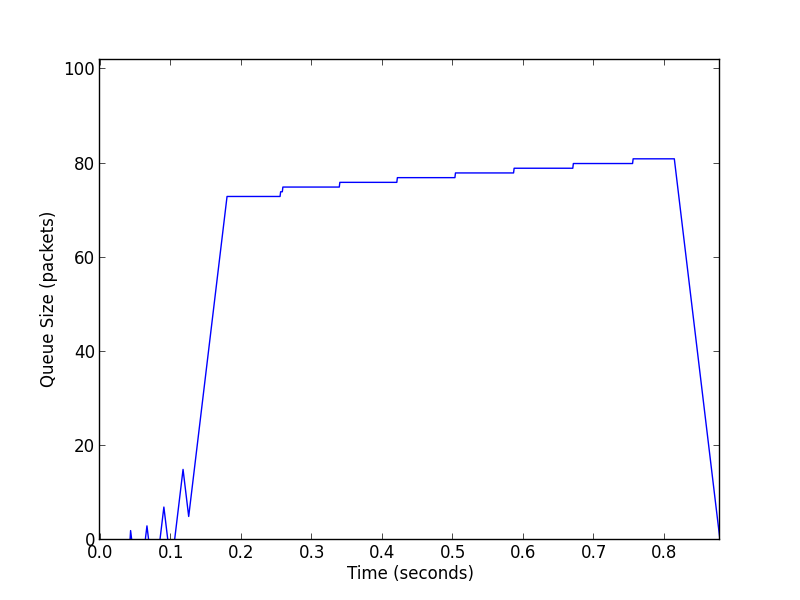
\includegraphics[width=13cm]{1_data/1-queue_q100}
\vspace{0.25cm}

\textit{Figure 3 - Receiver's Rate vs Time with Max Queue Size of 80}
\\
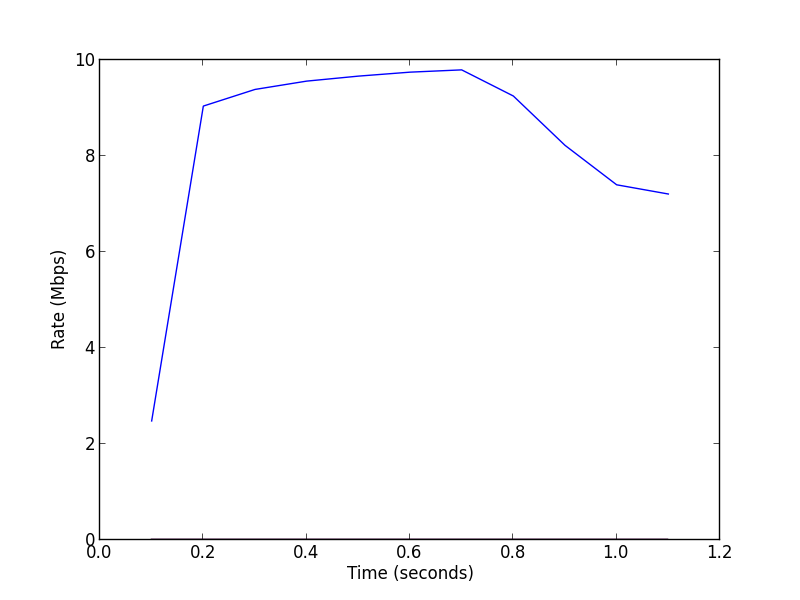
\includegraphics[width=13cm]{1_data/1-rate_q80}
\vspace{0.25cm}

\textit{Figure 4 - Receiver's Rate vs Time with Max Queue Size of 80}
\\
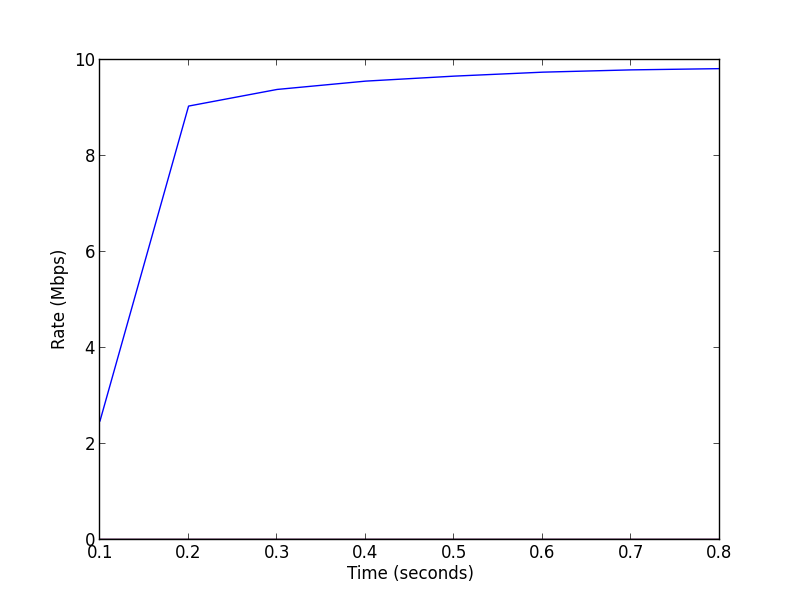
\includegraphics[width=13cm]{1_data/1-rate_q100}
\vspace{0.25cm}

\textit{Figure 5 - Congestion Window vs Time with Max Queue Size of 80}
\\
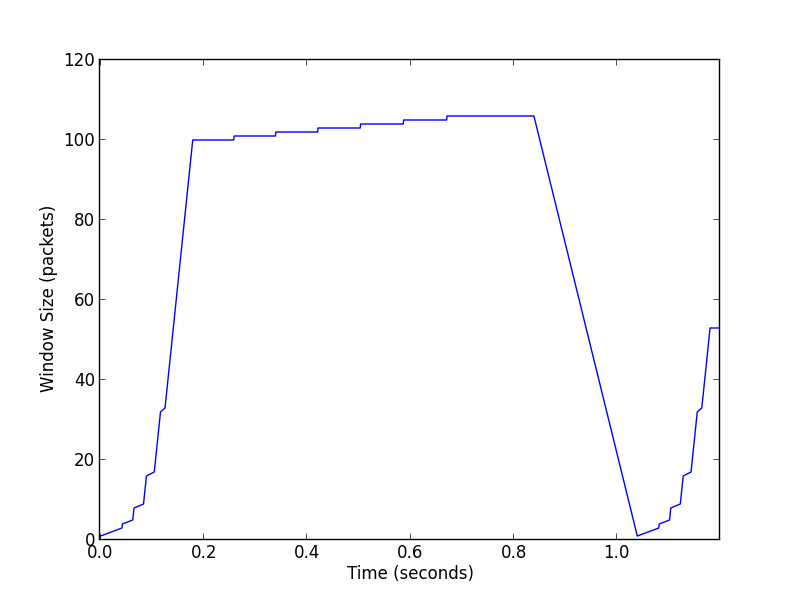
\includegraphics[width=13cm]{1_data/1-window_q80}
\vspace{0.25cm}

\textit{Figure 6 - Congestion Window vs Time with Max Queue Size of 80}
\\
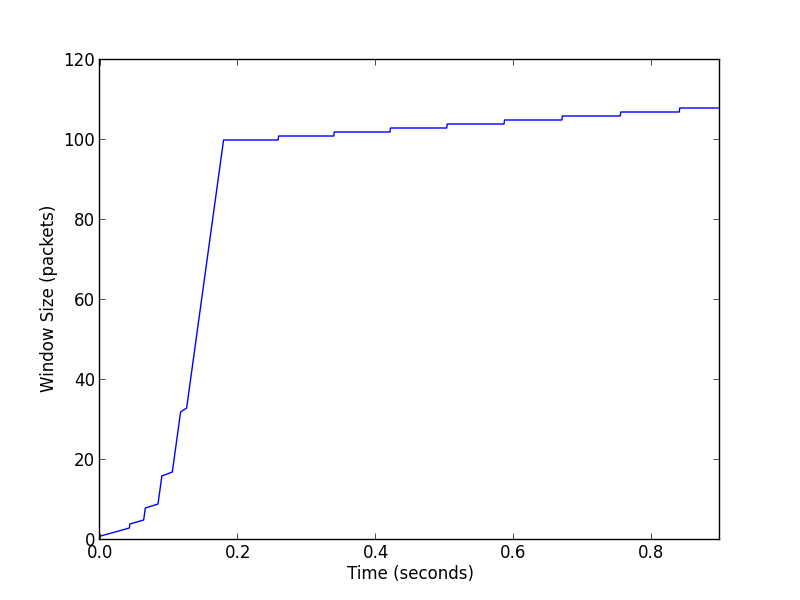
\includegraphics[width=13cm]{1_data/1-window_q100}
\vspace{0.25cm}

\textit{Figure 7 - Sequence No., ACK, and Packet Loss over Time with Max Queue Size of 80}
\\
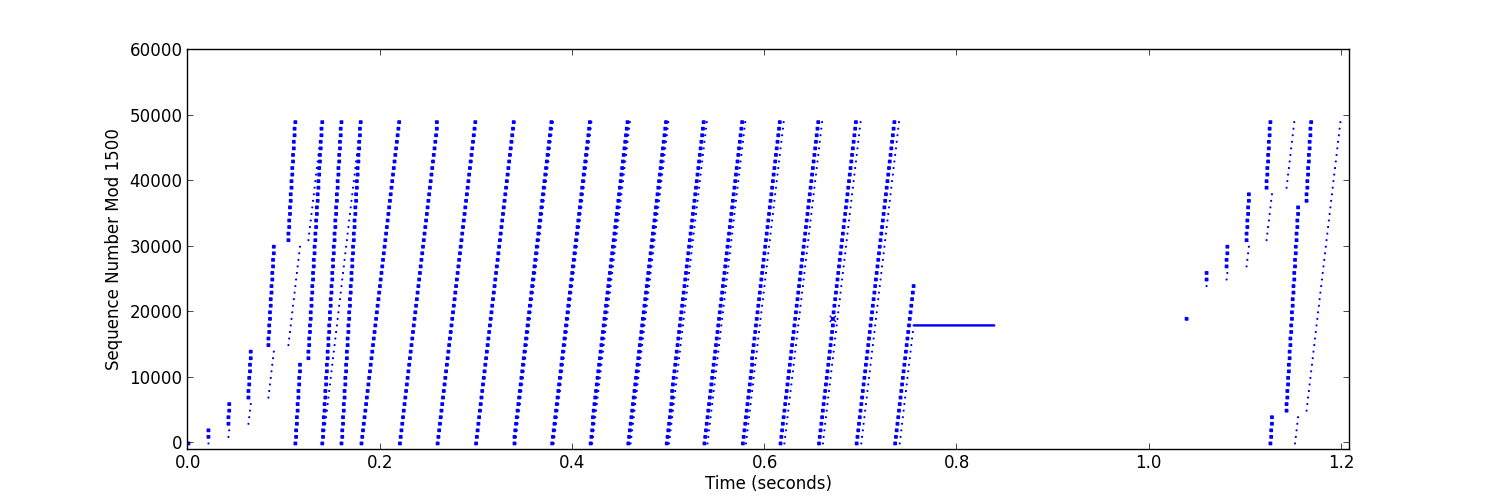
\includegraphics[width=18cm]{1_data/1-sequence_q80}
\vspace{0.25cm}

\textit{Figure 8 - Sequence No., ACK, and Packet Loss over Time with Max Queue Size of 100}
\\
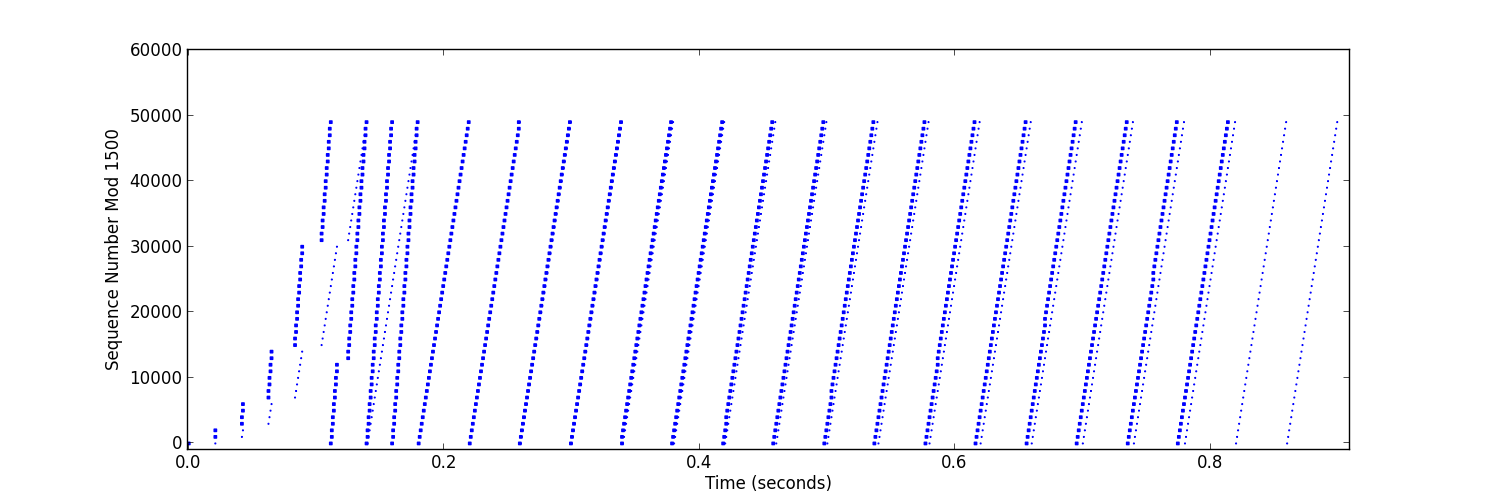
\includegraphics[width=18cm]{1_data/1-sequence_q100}
\vspace{0.25cm}

\textbf{Experiment 2} required that there be 2 flows accessing the network at the same time in order to perform a file transfer over each flow. The exported data for Experiment 2 is in the text files (\textit{.txt} extension) in the \textit{2\_data} directory. The plots created from the data are displayed as figures 9 through 13.
\vspace{0.25cm}
\textit{Figure 9 - 2 Flows, Queue Size vs Time}
\\
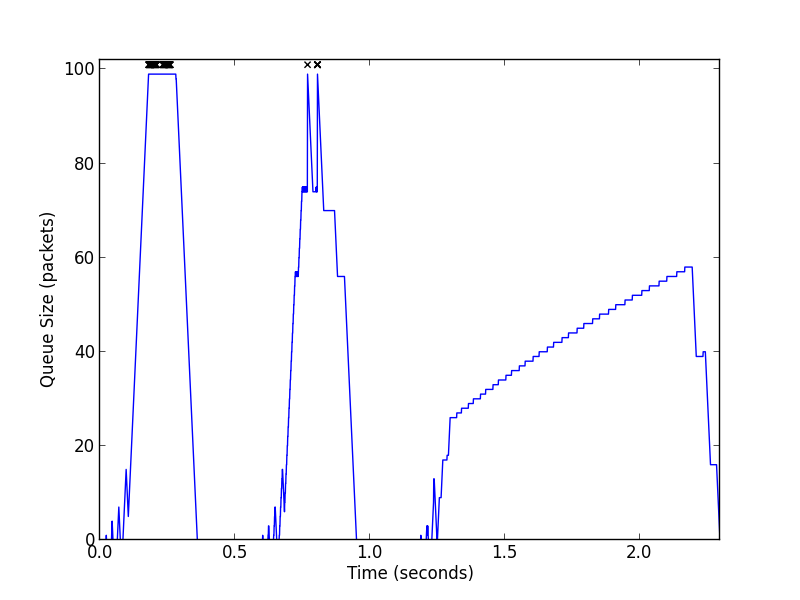
\includegraphics[width=13cm]{2_data/2-queue}
\vspace{0.25cm}

\textit{Figure 10 - 2 Flows, Receiver's Rate vs Time}
\\
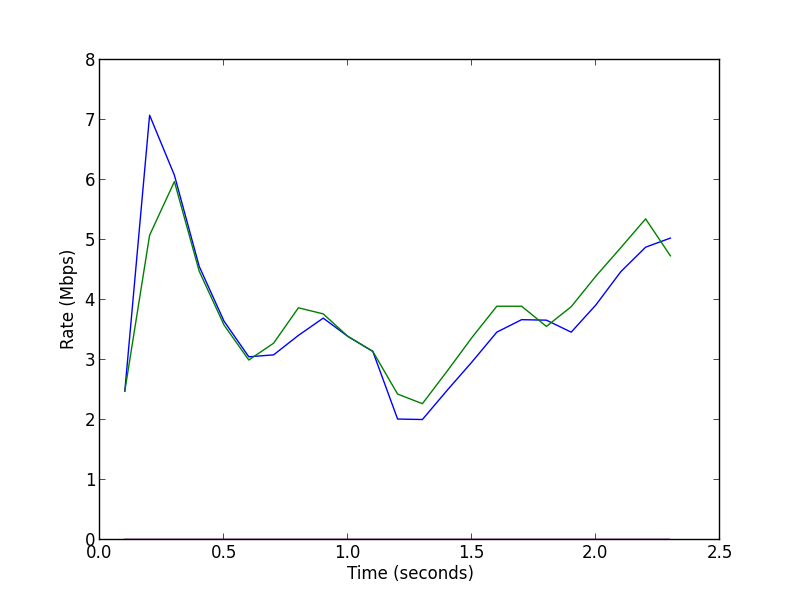
\includegraphics[width=13cm]{2_data/2-rate}
\vspace{0.25cm}

\textit{Figure 11 - 2 Flows, Flow 1 Congestion Window vs Time}
\\
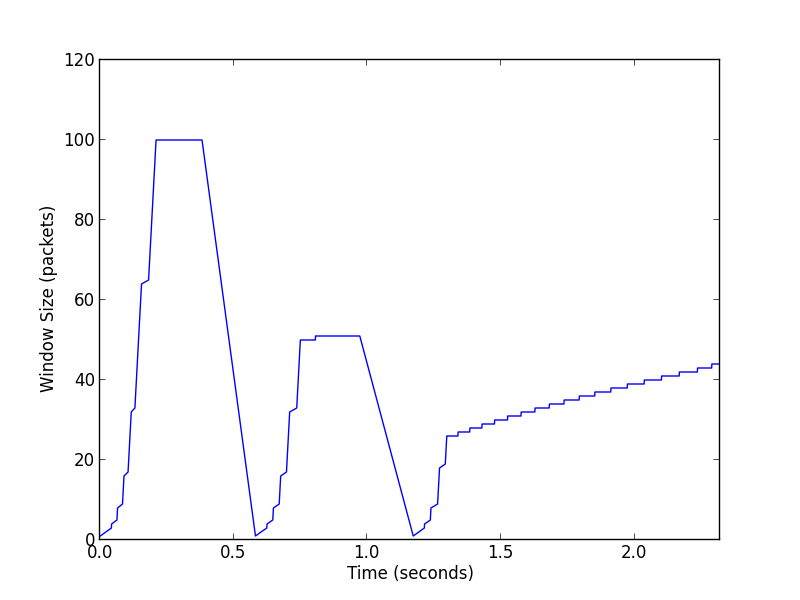
\includegraphics[width=13cm]{2_data/2_1-window}
\vspace{0.25cm}

\textit{Figure 12 - 2 Flows, Flow 2 Congestion Window vs Time}
\\
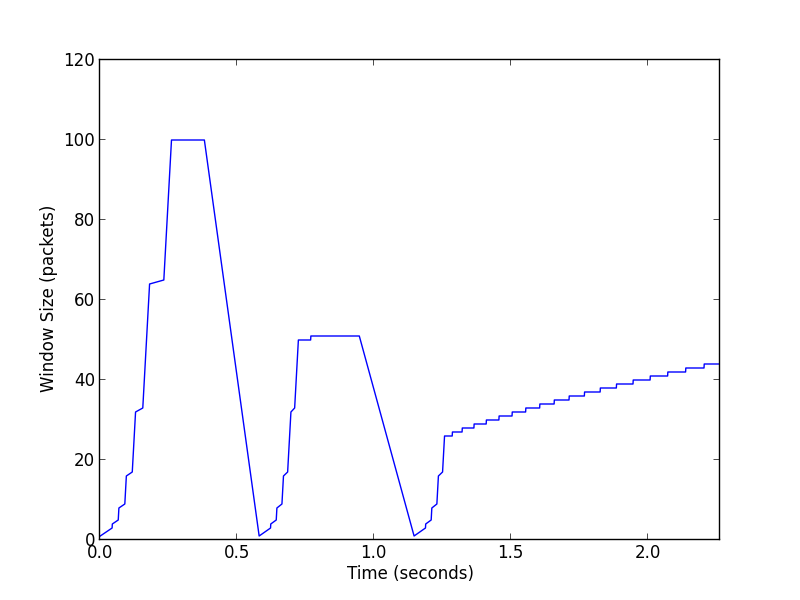
\includegraphics[width=13cm]{2_data/2_2-window}
\vspace{0.25cm}

\textit{Figure 13 - 2 Flows, Sequence No., ACK, and Packet Loss over Time}
\\
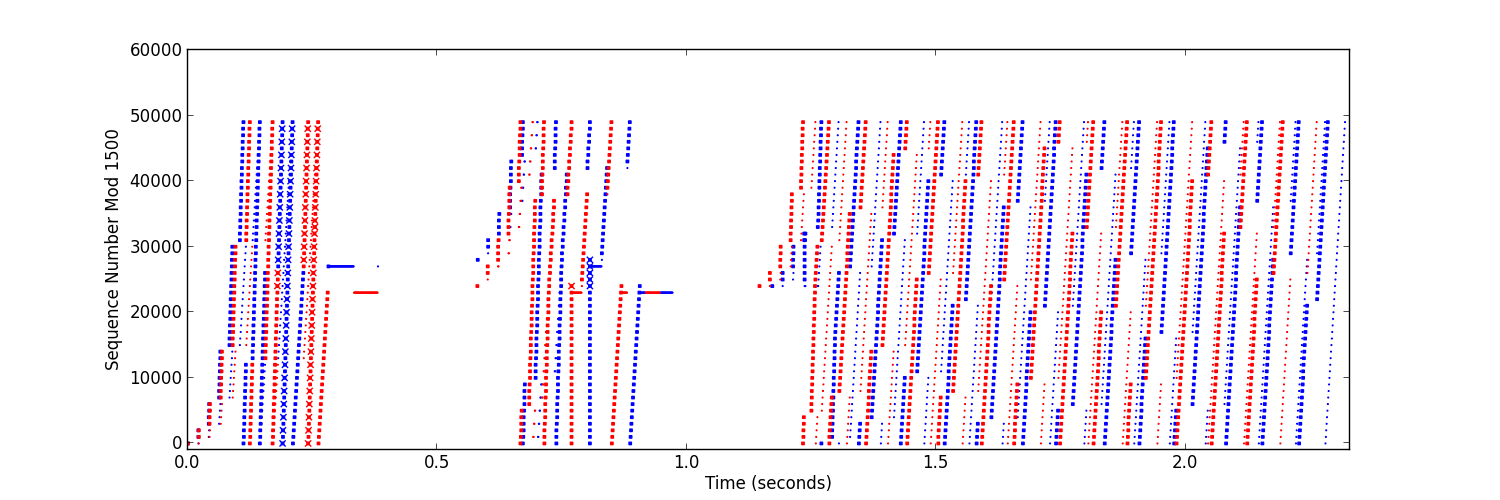
\includegraphics[width=18cm]{2_data/2-sequence}
\vspace{0.25cm}

\textbf{Experiment 5} used the same network set up as experiments 2 and 1, but this time there were five file transfers, and each one started at a different time in the Simulator. This is apparent in the data and on the graphs below. The data for experiment 5 is saved in the \textit{5\_data} directory. Figures 14 through 21 show the plots created from the data:

\vspace{0.25cm}
\textit{Figure 14 - 5 Flows, Queue Size vs Time}
\\
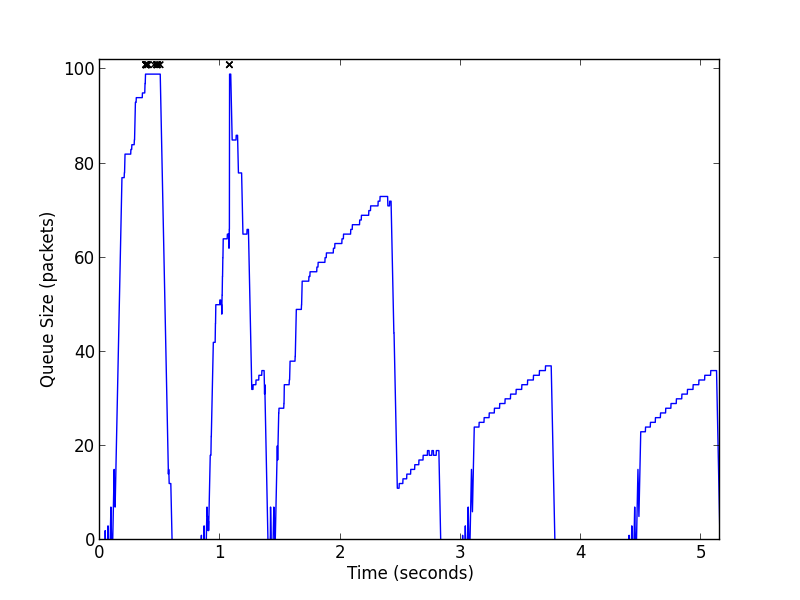
\includegraphics[width=13cm]{5_data/5-queue}
\vspace{0.25cm}

\textit{Figure 15 - 5 Flows, Receiver's Rate vs Time}
\\
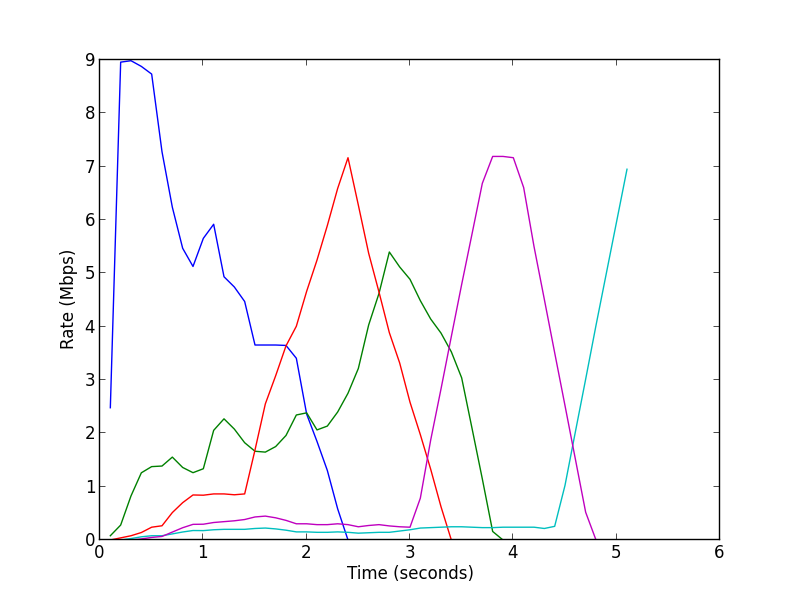
\includegraphics[width=13cm]{5_data/5-rate}
\vspace{0.25cm}

\textit{Figure 16 - 5 Flows, Flow 1 Congestion Window vs Time}
\\
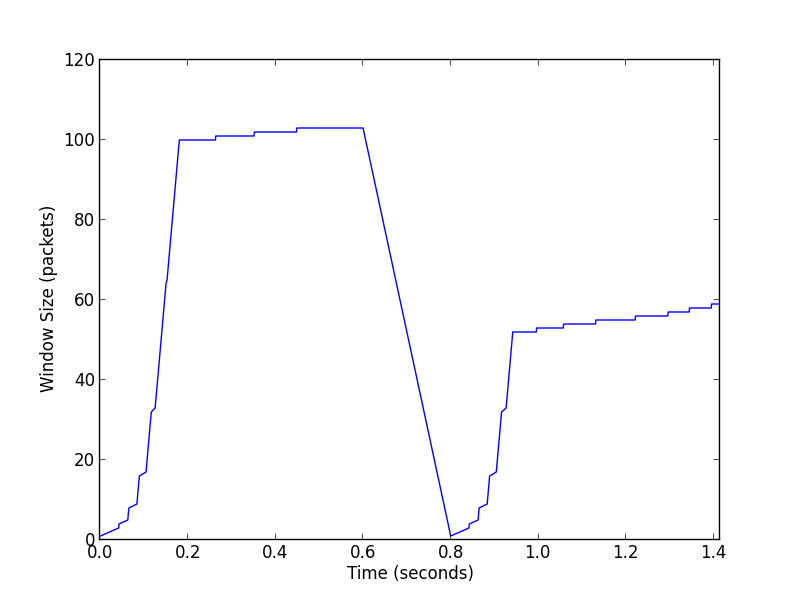
\includegraphics[width=13cm]{5_data/5_1-window}
\vspace{0.25cm}

\textit{Figure 17 - 5 Flows, Flow 2 Congestion Window vs Time}
\\
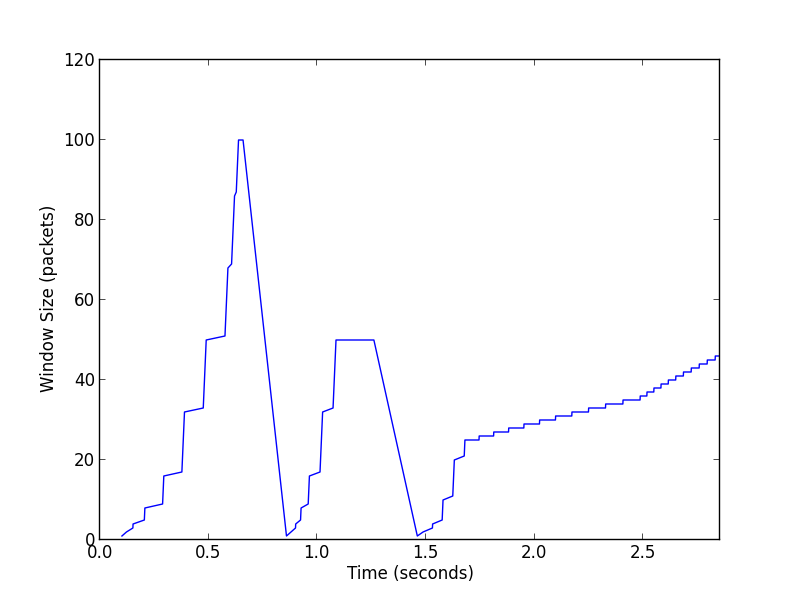
\includegraphics[width=13cm]{5_data/5_2-window}
\vspace{0.25cm}

\textit{Figure 18 - 5 Flows, Flow 3 Congestion Window vs Time}
\\
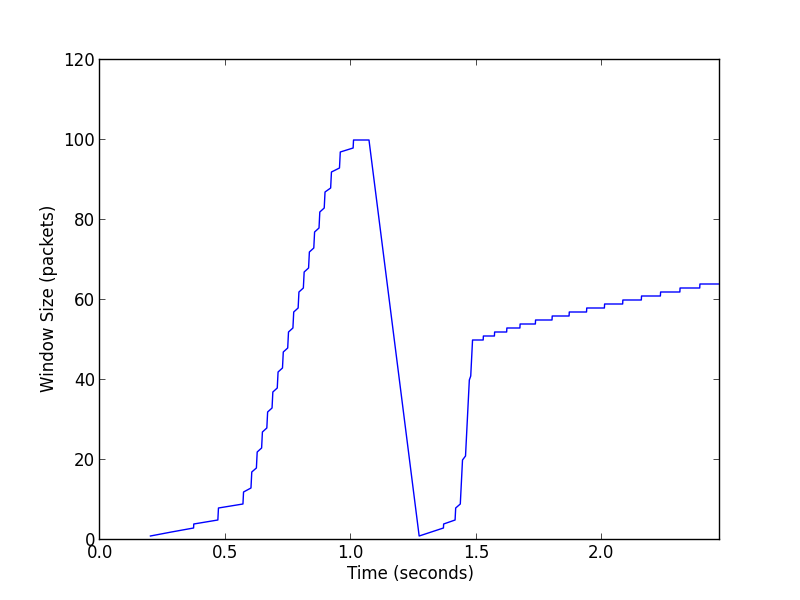
\includegraphics[width=13cm]{5_data/5_3-window}
\vspace{0.25cm}

\textit{Figure 19 - 5 Flows, Flow 4 Congestion Window vs Time}
\\
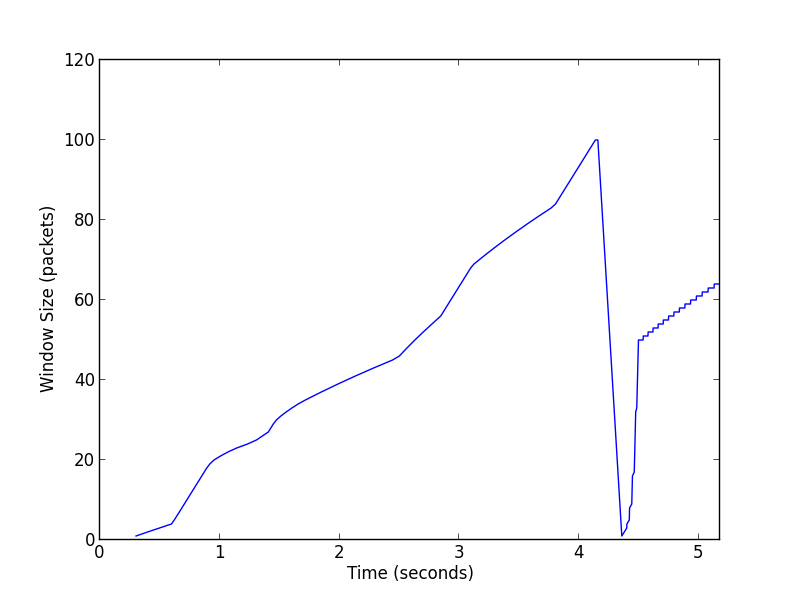
\includegraphics[width=13cm]{5_data/5_4-window}
\vspace{0.25cm}

\textit{Figure 20 - 5 Flows, Flow 5 Congestion Window vs Time}
\\
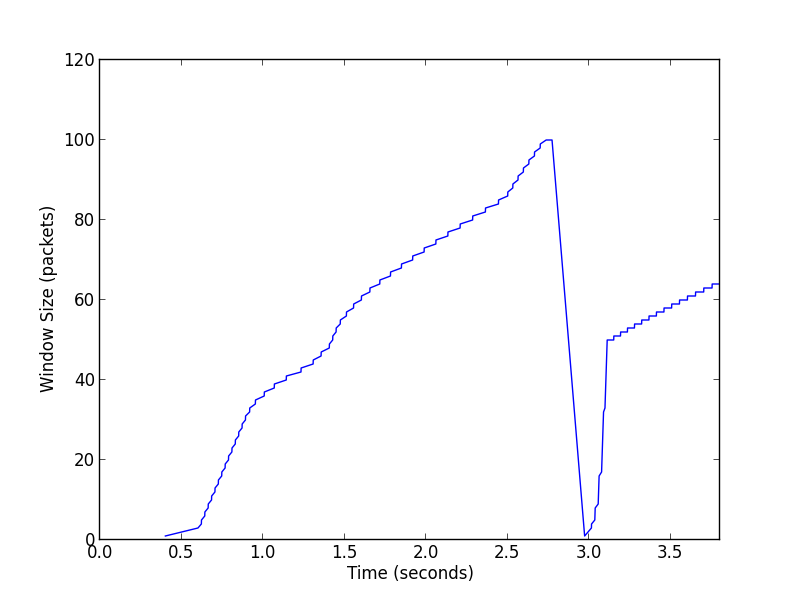
\includegraphics[width=13cm]{5_data/5_5-window}
\vspace{0.25cm}

\textit{Figure 21 - 5 Flows, Sequence No., ACK, and Packet Loss over Time}
\\
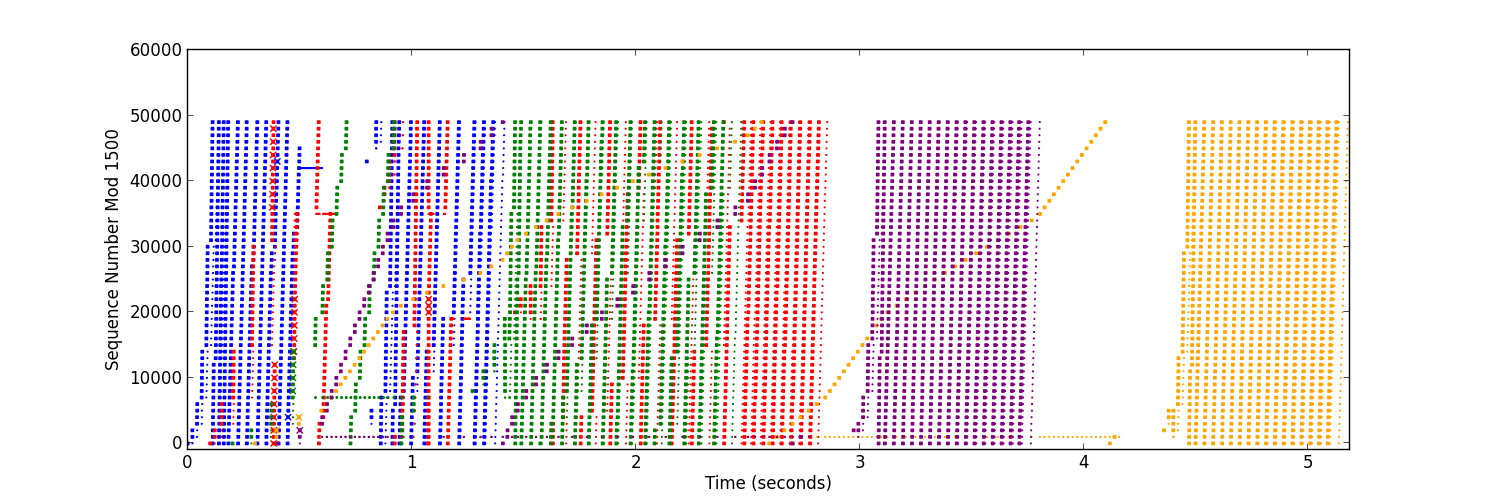
\includegraphics[width=18cm]{5_data/5-sequence}
\vspace{0.25cm}

\section{Conclusion}

After running the experiments, I believe that the data I collected shows that my implementation of TCP Tahoe is correct. The queue plots have the shape expected. The rate plots show the interaction between the multiple flows and how they are affected by each other. The window plots show the window sizes adjusting correctly. And the sequence plots are also correct.

\end{document}
